\documentclass[border=6pt]{standalone}
\usepackage{tikz}
\usetikzlibrary{arrows.meta,positioning,bending}

\definecolor{intfill}{RGB}{233,211,122}    % gold (internal nodes)
\definecolor{leaffill}{RGB}{200,216,242}   % light blue (external/leaf nodes)
\definecolor{nodeline}{RGB}{60,72,140}     % navy
\definecolor{elemcol}{RGB}{200,60,40}      % red element pointer
\definecolor{lettercol}{RGB}{150,70,30}    % brown element label

% A binary-tree node box: #1 x, #2 y, #3 fill, #4 left cell, #5 parent (top-mid),
% #6 right cell, #7 element letter
\newcommand{\btnode}[7]{%
  \begin{scope}[shift={(#1,#2)}]
    \fill[#3, rounded corners=5pt] (-1.2,-0.5) rectangle (1.2,0.5);
    \draw[nodeline, line width=1pt, rounded corners=5pt] (-1.2,-0.5) rectangle (1.2,0.5);
    \draw[nodeline, line width=0.8pt] (-0.4,-0.5) -- (-0.4,0.5);
    \draw[nodeline, line width=0.8pt] ( 0.4,-0.5) -- ( 0.4,0.5);
    \draw[nodeline, line width=0.8pt] (-0.4, 0.0) -- ( 0.4,0.0);
    \node[nodeline] at (-0.8,0)   {#4};
    \node[nodeline] at ( 0.8,0)   {#6};
    \node[nodeline] at ( 0,0.25)  {#5};
    \fill[elemcol] (0,-0.25) circle (1.6pt);
    \draw[elemcol, line width=1pt, -{Latex[length=2.4mm]}] (0,-0.27) -- (0,-1.05);
    \node[text=lettercol, font=\Large] at (0,-1.4) {#7};
  \end{scope}}

\begin{document}
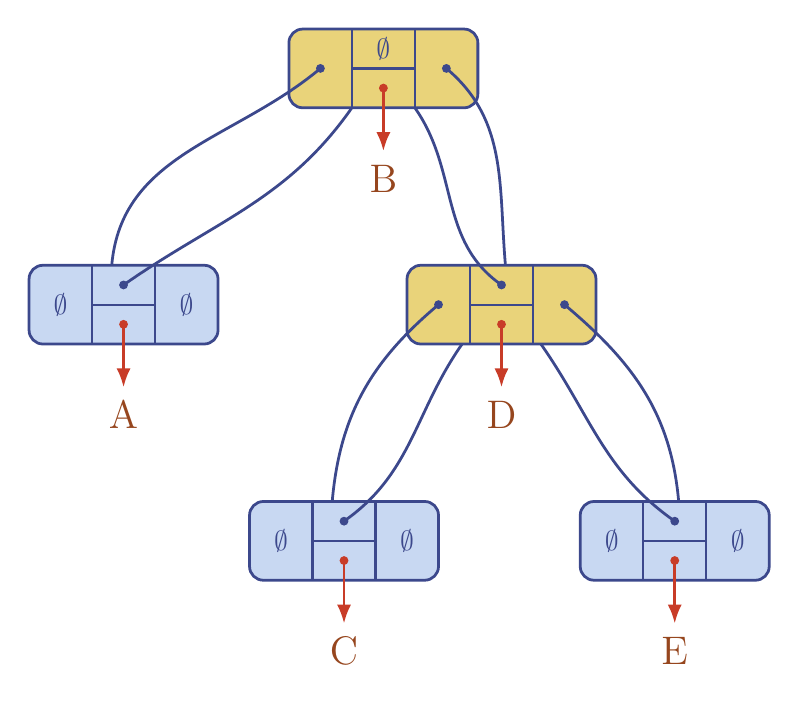
\begin{tikzpicture}[
  ptr/.style={draw=nodeline, line width=1pt},
]
% ---- Nodes ----
\btnode{4.5}{6.0}{intfill}{}{$\emptyset$}{}{B}      % root
\btnode{1.2}{3.0}{leaffill}{$\emptyset$}{}{$\emptyset$}{A}
\btnode{6.0}{3.0}{intfill}{}{}{}{D}
\btnode{4.0}{0.0}{leaffill}{$\emptyset$}{}{$\emptyset$}{C}
\btnode{8.2}{0.0}{leaffill}{$\emptyset$}{}{$\emptyset$}{E}

% ---- Child pointers: begin at the inner left/right field dots; bow outward ----
\foreach \px/\py in {3.7/6.0, 5.3/6.0, 5.2/3.0, 6.8/3.0}
  \fill[nodeline] (\px,\py) circle (1.6pt);
\draw[ptr] (3.7,6.0) to[out=-140,in=85]  (1.05,3.5);  % B.left  -> A
\draw[ptr] (5.3,6.0) to[out=-40,in=95]   (6.05,3.5);  % B.right -> D
\draw[ptr] (5.2,3.0) to[out=-140,in=85]  (3.85,0.5);  % D.left  -> C
\draw[ptr] (6.8,3.0) to[out=-40,in=95]   (8.25,0.5);  % D.right -> E

% ---- Parent pointers: begin at the inner parent field; bow the other way ----
\foreach \px/\py in {1.2/3.25, 6.0/3.25, 4.0/0.25, 8.2/0.25}
  \fill[nodeline] (\px,\py) circle (1.6pt);
\draw[ptr] (1.2,3.25) to[out=35,in=-125]  (4.1,5.5);   % A -> B
\draw[ptr] (6.0,3.25) to[out=145,in=-55]  (4.9,5.5);   % D -> B
\draw[ptr] (4.0,0.25) to[out=35,in=-125]  (5.5,2.5);   % C -> D
\draw[ptr] (8.2,0.25) to[out=145,in=-55]  (6.5,2.5);   % E -> D
\end{tikzpicture}
\end{document}
